\section{Pine Island Glacier Sensitivity Study}
\subsection{Goals} %{{{
This example is adapted from the results presented in \cite{Seroussi2014}. We model the impact of different external forcings on the dynamic evolution of Pine Island Glacier. The main objectives are to:
\begin{itemize}
	\item Run transient simulations (10 years) of a real glacier
	\item Change external forcings
	\item Compare the impact of changes on glacier dynamics and volume
\end{itemize}

Files needed to run this tutorial are located in \verb@trunk/examples/PigSensitivity/@. This tutorial relies on experience gained from completing the \href{http://issm.jpl.nasa.gov/documentation/tutorials/pig}{Pine Island Glacier} and \href{http://issm.jpl.nasa.gov/documentation/tutorials/greenland}{Greenland Ice Sheet} modeling tutorials, so make sure to complete them first.
%}}}
\subsection{Evolution over 10 years}%{{{
We first run a simulation of Pine Island Glacier over a 10 year period, starting from the \verb@Pig@ tutorial.

In the \verb@runme.m@ file, several parameters are adjusted before running the transient model. Open \verb@runme.m@ and make sure that the variable \verb@steps@, at the top of the file, is set to \verb@steps=[1]@. In the code, you will see that in step 1 the following actions are implemented:
\begin{itemize}
	\item Load model from the \verb@Pig@ tutorial
	\item Apply some basal melting rate
		\begin{itemize}
			\item On grounded ice: \verb@md.basalforcings.groundedice_melting_rate@
			\item On floating ice: \verb@md.basalforcings.floatingice_melting_rate@
		\end{itemize}
	\item Specify time step length and run duration in \verb@md.timestepping@
	\item Disable inverse method in \verb@md.inversion.iscontrol = 0@
	\item Indicate what components of the transient to activate
		\begin{itemize}
			\item \verb@md.transient.ismasstransport@
			\item \verb@md.transient.isstressbalance@
			\item \verb@md.transient.isthermal@
			\item \verb@md.transient.isgroundingline@
			\item \verb@md.transient.ismovingfront@
		\end{itemize}
	\item Request additional outputs
	\item Solve transient solution
\end{itemize}

Execute \verb@runme@ to perform step 1. The following figure shows the evolution of the ice velocity and grounding line positions at the beginning and at the end of the simulation:
\begin{figure}[H]
	\begin{center}
		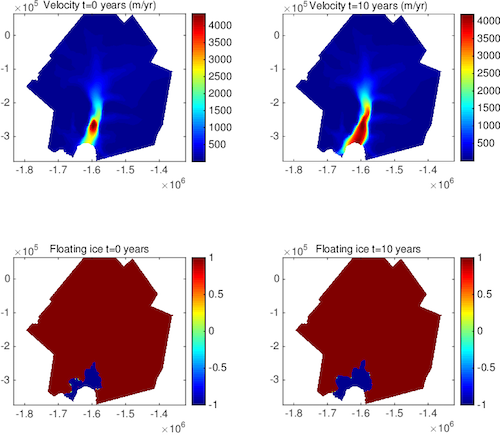
\includegraphics[scale=0.9]{/assets/img/using-issm/tutorials/pigsensitivity/ResultsTransient.png}
	\end{center}
\end{figure}
%}}}
\subsection{Increased basal melting rate}%{{{
In this second step, we increase the basal melting rate under the floating portion of the domain from 25 to 60 m/yr. The other parameters remain the same as in the previous step.

Open \verb@runme.m@ and change the step at the top of the file to \verb@step=2@, then run the simulation. The following figure shows the evolution of ice velocity and grounding line evolution for the increased melting scenario:
\begin{figure}[H]
	\begin{center}
		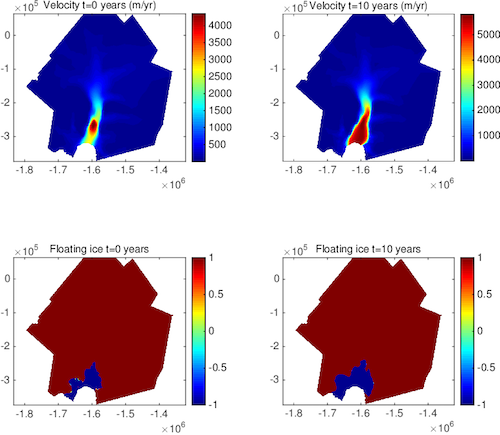
\includegraphics[scale=0.9]{/assets/img/using-issm/tutorials/pigsensitivity/ResultsHighMelt.png}
	\end{center}
\end{figure}
%}}}
\subsection{Retreat of ice front position}%{{{
In this third step, we would like to test the sensitivity of Pig to calving events and retreat the position of the ice front. We first need to create a new contour of the region to be removed from the domain. Use \verb@exptool@ to create a new \verb@RetreatFront.exp@ contour that include the portion of floating ice that should calve off.

Then extract the domain from the initial model, excluding the \verb@RetreatFront.exp@ area using the \verb@extrude@ routine:
\begin{verbatim}>> md2=modelextract(md,~RetreatFront.exp)\end{verbatim}

As this operation changes the model domain, some parameters and boundary conditions have the be adjusted or redefined.

The boundary conditions are reset with \verb@SetMarineIceSheetBC@ and the model can then be solved.

Open \verb@runme.m@ and change the step at the top of the file to \verb@step=3@, then run the simulation. The following figure shows the evolution of ice velocity and grounding line evolution with the new ice front:
\begin{figure}[H]
	\begin{center}
		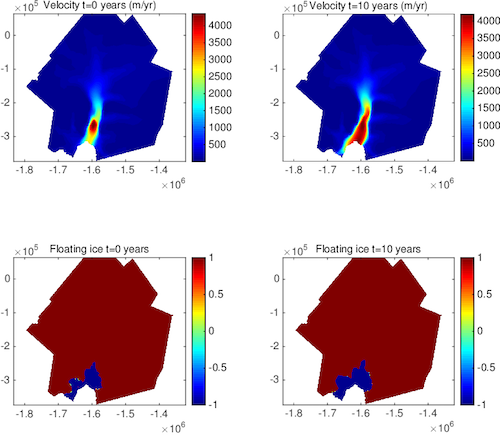
\includegraphics[scale=0.9]{/assets/img/using-issm/tutorials/pigsensitivity/ResultsFrontRetreat.png}
	\end{center}
\end{figure}
%}}}
\subsection{Change in surface mass balance}%{{{
In this last step, we change the surface mass balance, while the other parameters remain similar to the previous simulations.

Open \verb@runme.m@ and implement the changes needed to investigate the impact of the surface mass balance, similar to what was done with the other external forcings in the previous steps. These changes are:
\begin{itemize}
	\item Load model from the \verb@Pig@ tutorial
	\item Change the surface mass balance
	\item Verify the ocean-induced melting rate
		\begin{itemize}
			\item On grounded ice: \verb@md.basalforcings.groundedice_melting_rate@
			\item On floating ice: \verb@md.basalforcings.floatingice_melting_rate@
		\end{itemize}
	\item Specify time step length and run duration in \verb@md.timestepping@
	\item Disable inverse method in \verb@md.inversion.iscontrol@
	\item Indicate what components of the transient to activate
		\begin{itemize}
			\item \verb@md.transient.ismasstransport@
			\item \verb@md.transient.isstressbalance@
			\item \verb@md.transient.isthermal@
			\item \verb@md.transient.isgroundingline@
			\item \verb@md.transient.ismovingfront@
		\end{itemize}
	\item Request additional outputs
	\item Solve transient solution
\end{itemize}

Don't forget to change \verb@step@ at the top of the \verb@runme.m@.

Below is the solution to make this change:
\begin{verbatim}if step==4
	%Load model
	md = loadmodel('./Models/PIG_Transient');

	%Change external forcing basal melting rate and surface mass balance)
	md.basalforcings.groundedice_melting_rate=zeros(md.mesh.numberofvertices,1);
	md.basalforcings.floatingice_melting_rate=25*ones(md.mesh.numberofvertices,1);
	md.smb.mass_balance=2*md.smb.mass_balance;

	%Define time steps and time span of the simulation
	md.timestepping.time_step=0.1;
	md.timestepping.final_time=10;

	%Request additional outputs
	md.transient.requested_outputs={'default','IceVolume','IceVolumeAboveFloatation'};

	%Solve
	md=solve(md,'Transient');

	%Plot
	plotmodel(md, 'data', md.results.TransientSolution(1).Vel,...
		'title#1', 'Velocity t=0 years (m/yr)',...
		'data', md.results.TransientSolution(end).Vel,...
		'title#2', 'Velocity t=10 years (m/yr)',...
		'data', md.results.TransientSolution(1).MaskOceanLevelset,...
		'title#3', 'Floating ice t=0 years',...
		'data', md.results.TransientSolution(end).MaskOceanLevelset,...
		'title#4', 'Floating ice t=10 years',...
		'caxis#1',([0 4500]),'caxis#2',([0 4500]),...
		'caxis#3',([-1,1]),'caxis#4',([-1,1]));

	%Save model
	save ./Models/PIG_SMB md;
end\end{verbatim}

Here is an example of velocity change and grounding line evolution when the surface mass balance is doubled:
\begin{figure}[H]
	\begin{center}
		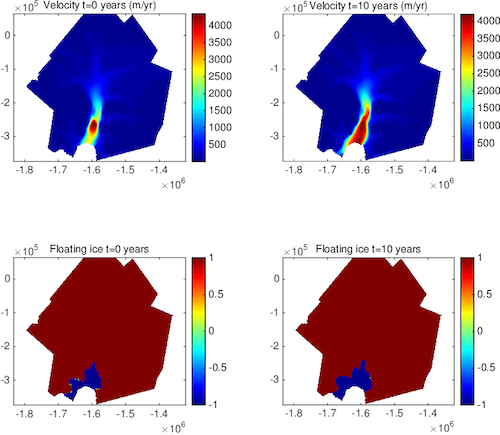
\includegraphics[scale=0.9]{/assets/img/using-issm/tutorials/pigsensitivity/ResultsSMB.png}
	\end{center}
\end{figure}
%}}}
\subsection{Evolution of the ice volume above flotation} %{{{
In the previous steps, we investigated the impact of changes in external forcings on ice flow dynamics (grounding line evolution and glacier acceleration). We can also see how these changes impact the glacier volume and its contribution to sea level rise. To do so, we use the additional output \verb@IceVolumeAboveFloatation@ requested in the transient simulation. The following figure shows the evolution of the volume (in Gt/yr) above flotation for the four scenarios performed previously:
\begin{figure}[H]
	\begin{center}
		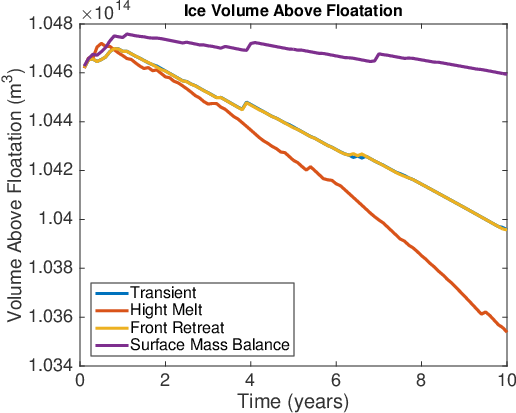
\includegraphics[scale=0.9]{/assets/img/using-issm/tutorials/pigsensitivity/EvolutionVAF.png}
	\end{center}
\end{figure}
%}}}
